% This is samplepaper.tex, a sample chapter demonstrating the
% LLNCS macro package for Springer Computer Science proceedings;
% Version 2.20 of 2017/10/04
%
\documentclass[runningheads]{llncs}
%
\usepackage{graphicx}
\usepackage{tikz}
\usepackage{pgfplots}
\pgfplotsset{compat=1.17}

%\usepackage{amsmath,amsthm,amsfonts,amssymb,latexsym}
\usepackage{amsmath,amsfonts,amssymb,latexsym}
% Used for displaying a sample figure. If possible, figure files should
% be included in EPS format.
%
% If you use the hyperref package, please uncomment the following line
% to display URLs in blue roman font according to Springer's eBook style:
% \renewcommand\UrlFont{\color{blue}\rmfamily}

\begin{document}
%
\title{Optimizacion de distribucion de antenas de telecomunicaciones}
%
%\titlerunning{Abbreviated paper title}
% If the paper title is too long for the running head, you can set
% an abbreviated paper title here
%
\author{Integrantes:\\ Carlos Garcia y Sebastian Pinzon \\
	\textbf{Entrega 1:Primera aproximaci\'{o}n del Modelo Matem\'{a}tico  \\Modelado, Simulaci\'{o}n y Optimizaci\'{o}n} \\}
%
\authorrunning{Garcia, Pinzon}
% First names are abbreviated in the running head.
% If there are more than two authors, 'et al.' is used.
%
\institute{Departamento de Ingenier\'{i}a de Sistemas y Computaci\'{o}n \\
	Universidad de Los Andes\\
	Bogot\'{a}, Colombia}
%
\maketitle              % typeset the header of the contribution
%
%
%
%
%\\
%Nombre:\\
\section{Descripci\'{o}n del Problema}
En el mundo de las telecomunicaciones mantener conectados a los ususarios en la prioridad numero 1, sin embargo la infraestructura requiridad para esto puede llegar a ser muy costosa. Con esto en mente la optimizacion de la cobertura de las antenas usadas para conectar a los usuarios es muy importante. Las empresas tienen acceso a diferentes tipos de antenas con diferentes costos y diferents coberturas. Nuestro trabajo sera encontrar la manera de posicionar las antenas en un plano, maximizando cobertura y minimizando costos.
\\ \\
A pesar de que intentamos resolver un problema real, debemos tener en cuenta ciertas restricciones para la simplicidad del problema. Primero no tendremos en cuenta ni topologia ni logistica, en el mundo real hay contrucciones en ciertos lugares que no nos dejarian poner las antenas o caracteristicas geograficas que dificultan este proceso, como montañas o tereno inestable. Tambien tendros que ignorar aspectos tecnicos como interferencia de otras antenas. Sin embargo estas omiciones aun nos permiten extraer informacion valiosa para mejorar estos sistemas.
\\ \\
\begin{figure}
	\centering
	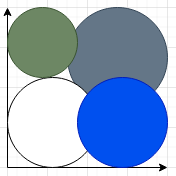
\includegraphics[width=0.25\textwidth]{plot3.png}
	\caption{Ejemplo de los radios que ocuparian las antenas}
	\label{fig:your-image}
\end{figure}
\\






\section{Conjuntos, Par\'{a}metros y Variables}

\begin{table}[h]
	\caption{Conjuntos y Par\'{a}metros. \label{Tab: tab1}}
	\begin{tabular*}{\hsize}{@{\extracolsep{\fill}}ll@{}}
		\hline
		\textbf{Sets and Parameters} & \textbf{Description}\\
		\hline
		T & Tipos de antena.\\
		$X$  & Posibles coordenadas en el eje X.\\
		$Y$  & Posibles coordenadas en el eje Y.\\
		\hline
	\end{tabular*}
\end{table}

% Table 1, part 2
\begin{table}[h]
	\caption{Variables de decisi\'{o}n}
	\begin{tabular*}{\hsize}{@{\extracolsep{\fill}}ll@{}}
		\hline
		\textbf{Variables} & \textbf{Description}\\
		\hline
		$A_{xy}^t$ & Determina si en la coordenada x,y se encuentra una\\
		& antena de tipo t.\\
		$P_{x,y}$ & Determina si el punto x,y tiene almenos una antena en\\
		& rango\\
		$R_{t}$ &   Determina el radio de cobertura de una antena tipo t.\\
		$C_{t}$  & Determina el costo de la antena tipo t. \\
		\hline
	\end{tabular*}
\end{table}

\newpage
\section{Funci\'{o}n Objetivo y Restricciones.}

\begin{equation}
	F.O 1: min (\sum_{y \in Y} \sum_{x \in X} \sum_{t \in T} C_{ij} A_{xy}^t)
\label{eq:res1}
\end{equation}

\begin{equation}
	F.O 2: max (\sum_{y \in Y} \sum_{x \in X} P_{xy})\label{eq:res2}
\end{equation}


La F.O 1 Nos indica que debemos minimizar el costo total de la red de antenas, se revisa cuantas antenas hay y se multiplican por el costo de su tipo.
\\

La F.O 2 Nos indica que debemos maximizar la cantidad de coordenadas con cobertura.
\\
\\

%
% ---- Bibliography ----
%
% BibTeX users should specify bibliography style 'splncs04'.
% References will then be sorted and formatted in the correct style.
%
% \bibliographystyle{splncs04}
% \bibliography{mybibliography}
%

\end{document}
